\section{Selecting an External Planner}
As discussed in my design I will be creating a wrapper around an existing
external planner to collect together domain extensions and a problem to use as
input to the planner. SHOP2 (Simple Hierarchical Ordered Planner) is a
domain-independent automated planner, and the JSHOP2 (see appendix
\ref{appendix:JSHOP2}) implementation has great documentation (see reference
\cite{Ilghami2006}) as well as being free and open source is the perfect
external planner for my needs. Because it is a domain-independent planner it
accepts inputs of the domain and problem which describe the problem to solve as
well as the context (or domain) in which it should be solved. JSHOP2 expects
these input to be expressed in it's own planning domain definition language,
this is useful because I can modify the syntax of this language to allow for
domain extensions while still keeping the expressive power of the language.
Using JSHOP2's domain language also has the benefit of making it easier to
transform from my modified version to the version that JSHOP2 can process with
few errors.

\section{Parsing and Encoding}
The first part of my core design is to read domain extension and a problem
specifications supplied by the user. For this I needed to specify a domain and
problem language, luckily JSHOP2's documentation \citep{Ilghami2006} includes a
full definition of the data structures that make up domain language. To parse
the domain language and then encode it into a form that the JSHOP2 planner would
recognize I wrote three modules of code: a parser to initial parse and verify
that the domain extensions and problem are of the correct form; a pre-compiler
to process the representation produced by the parser into an internal
representation that is easier to work with; and an encoder which takes the
internal representation for the domain-extensions and parser and produces the
domain language that JSHOP2 recognizes.

\subsection{Parser}
Because SHOP2's original implementation is written in lisp, JSHOP2's domain
language takes heavy influence from lisp. This ends up being very useful when
parsing the language because I chose to implement the JSHOP2, wrapper in a lisp
family language called `Clojure' (see appendix \ref{appendix:clojure}). What
this means is, to read the domain extensions and problems I can just use the
`read-string' function provided by the language. By using functions included in
the language itself I can even get the added benefit of ignoring comments which
is a feature present in JSHOP2's specification with no extra effort.

To parse the domain-extensions and problem I used a Clojure library called
`clojure.spec' (see appendix \ref{appendix:clojure-spec}), this library allows
you to specify how a piece of data should be structured and any predicates that
the should be true for the data. This ends up being very similar to how JSHOP2's
documentation describes the domain language, because of this the parser is very
similar to the original JSHOP2 documentation.

\subsubsection{Differences to JSHOP2}
While writing the parser for the domain language I introduced a few minor
differences to the domain language to help increase readability of the language.
I have detailed these below:

\begin{itemize}
\item The `assign' keyword used for assignment is now `def', this is more
  similar to how clojure defines variables.
\item Task lists are vectors instead of list, this means that they use square
  brackets `[,]' instead of ordinary brackets `(,)'. This helps to differentiate
  them as a data structure.
\item Delete lists and add lists are also vectors.
\item Conjunctions now \emph{must} begin with an `and' keyword, unless they
  contain no expressions in which case they may be an empty list. This helps to
  distinguish between lists and conjunctions even further.
\item There is no way to specify a `domain', instead a vector of `axioms',
  `operators' and `methods' must be specified as a domain extension. These
  domain extensions will later be combined to form a single domain.
\item A problem does not specify what domain it will use as it is assumed that
  the domain will be the one created by merging the domain extensions.
\end{itemize}

\subsection{Pre-compiler}
The parser validates that the domain extensions and problem is of the correct
form, but it does not produce an output that is not easy to process. Because of
this a pre-compiler is needed to process the output of the parser into a form
that is easy to then encode into the form that JSHOP2 can understand. The
internal representation is similar in structure to how the language is defined,
each form stores information related to itself and it's children, but doesn't
store anything related to it's parent. The internal representation is defined
using a clojure data structure called a `record', this record is a map of keys
and values with some extra properties that allow for groups of functions call
`protocols' to quickly dispatch (choose the correct function to call) on.

\subsection{Encoder}
Because the internal representation is a nested structure of records (which can
be thought of as typed map or dictionaries in other languages), this allows me
to write the encoder in a way so that each records `knows' how to encode itself
using a protocol and can just recursively call the encode function on each of
it's children, if any, to build up it's encoded version. Because of this
property it was very easy to write the encoder part of the core, as I just had
to know how each type component in the domain language was expressed in JSHOP2's
language and write that out as a quoted form then finally serialize the newly
converted domain and problems into files for use in the external planner.

\section{Wrapping JSHOP2}
JSHOP2's planning process has 3 main stages to it: compiling the domain and
problem; recompiling the problem file; and finally running the problem to find a
plan. To properly `wrap' JSHOP2 I had to be able to execute this functionality
and read the results from within the core of my design.

\subsection{Calling JSHOP2}
Clojure is a language that runs on the Java Virtual Machine (JVM), this allows
clojure to offer interoperability with java code. I used this `interop' to call
the function that compiles the domain and problem files inputting the files
generated in the previous steps.

\subsection{Recompiling the Problem File}
JSHOP2 compiles it's domain and problem files into java source code that needs
to be compiled before it can be run, this requires that the java compiler be run
with the files produced by the previous step as inputs. The easiest way to do
this I found was to use the clojure library `clojure.shell' (see appendix
\ref{appendix:clojure-shell}) which allows me to make calls to the command line
of the operating system. Using clojure.shell I simply called the java compiler
`javac' to compile the problem file as specified in JSHOP2's documentation.

\subsection{Parsing JSHOP2's Output}
Once the problem file has been compiled it can simply be run using the
clojure.shell library and executing the compiled java files. The planners output
simply contains a line stating whether any plans were found or not, and if a
plan was found then it states a task list that would solve the problem specified
and a cost for the plan. These are simply parsed as strings and printed to the
user.

\begin{figure}
  \centering
  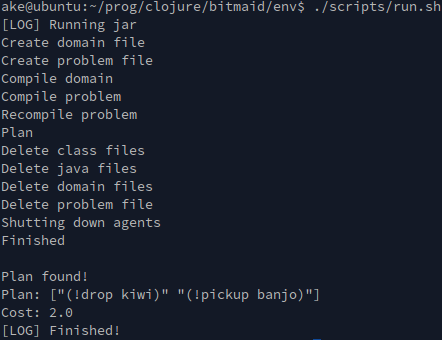
\includegraphics[width=0.6\linewidth]{figures/core-output.png}
  \caption{An example of a simple domain and problem being solved using the core
    and external planner.}
  \label{fig:core-example-output}
\end{figure}

%%% Local Variables:
%%% mode: latex
%%% TeX-master: "../diss"
%%% End: